\section{Đặc tả chi tiết Web hệ thống GPS Target Calculating System}
\begin{figure}[H]
    \centering
    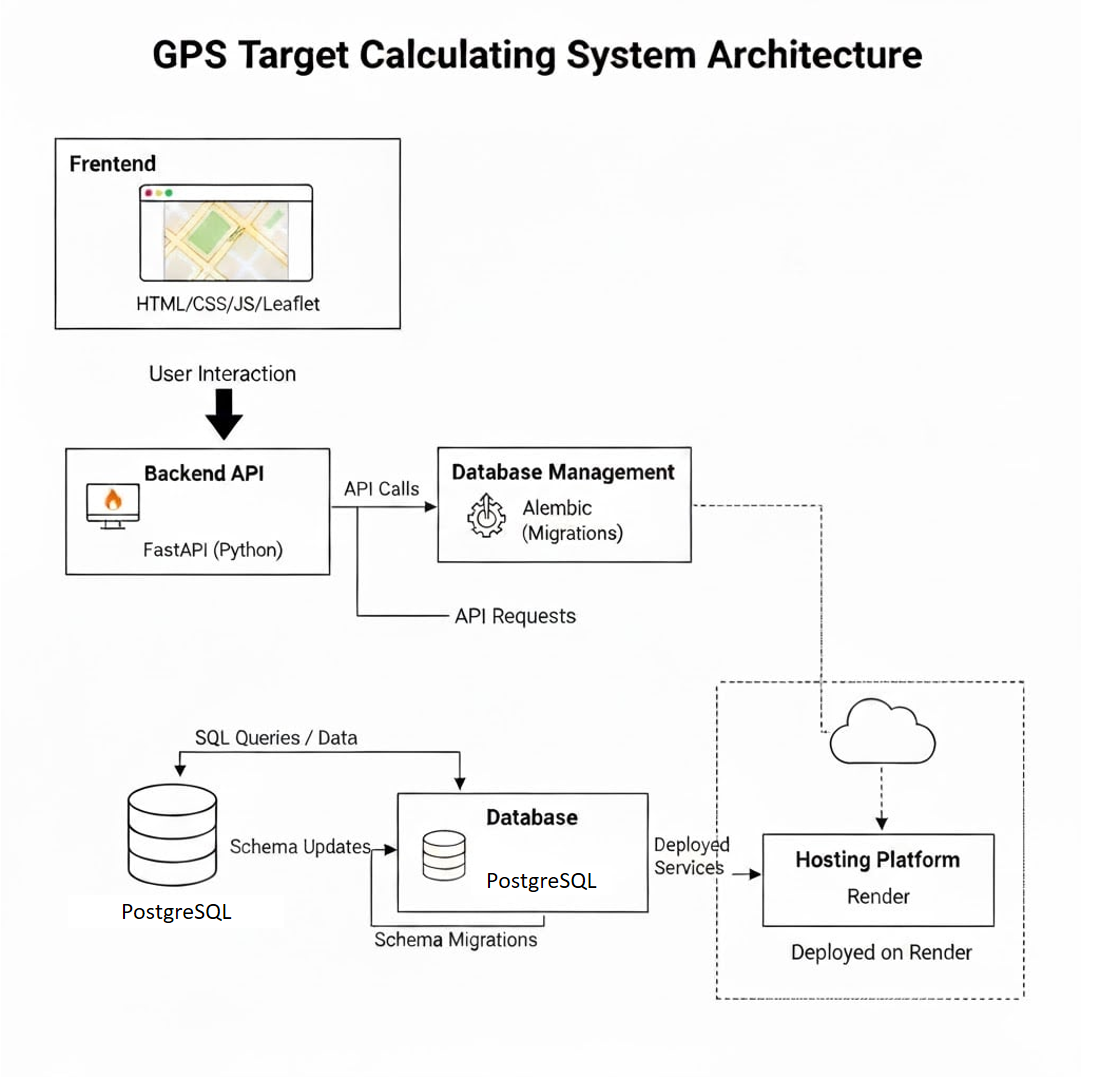
\includegraphics[scale=0.5]
    {Images/WebAr.png}
    \vspace{0.3cm} 
    \caption{Kiến trúc prototype của Web}
\end{figure}

\subsection{Tổng quan}
Hệ thống GPS Target Calculating System được thiết kế để tính toán và hiển thị vị trí mục tiêu dựa trên tọa độ người quan sát, góc ngắm và khoảng cách. Hệ thống bao gồm bốn thành phần chính: Frontend, Backend API, Database và Hosting Platform.
\subsection{Frontend (Giao diện người dùng)}
\begin{itemize}
    \item Công nghệ sử dụng: HTML, CSS, JavaScript, Leaflet.
    \item Chức năng chính:
    \begin{itemize}
        \item Hiển thị bản đồ tương tác bằng thư viện Leaflet.
        \item Cho phép người dùng nhập dữ liệu: tọa độ quan sát viên, góc ngắm, khoảng cách.
        \item Gửi dữ liệu này đến Backend API thông qua các lệnh gọi fetch() hoặc axios.
        \item Nhận kết quả tọa độ mục tiêu từ API và hiển thị marker trên bản đồ.
    \end{itemize}
    \item Đây là nơi người dùng trực tiếp thao tác; mọi tính toán phức tạp được ẩn đi và chỉ trả về kết quả trực quan.
\end{itemize}
\newpage
\subsection{Backend (FastAPI)}
\begin{itemize}
    \item Công nghệ sử dụng: Python, FastAPI.
    \item Cấu trúc chính:
    \begin{itemize}
        \item main.py: điểm khởi chạy ứng dụng, cấu hình CORS, đăng ký router.
        \item routers/calculate.py: định nghĩa endpoint /api/calculate để nhận dữ liệu và trả kết quả.
        \item models.py: định nghĩa bảng dữ liệu (Observation).
        \item schemas.py: định nghĩa input/output bằng Pydantic.
        \item database.py: cấu hình kết nối PostgreSQL.
        \item crud.py: các hàm thao tác với database.
    \end{itemize}
    \item Chức năng chính:
    \begin{itemize}
        \item Nhận dữ liệu từ FE (tọa độ, góc, khoảng cách).
        \item Tính toán tọa độ mục tiêu bằng công thức toán học.
        \item Lưu dữ liệu vào Database.
        \item Trả kết quả về cho FE qua JSON.
    \end{itemize}
    \item Đây là “bộ não” của hệ thống, xử lý logic nghiệp vụ và kết nối dữ liệu.
\end{itemize}

\subsection{Database (PostgreSQL + Alembic)}
\begin{itemize}
    \item Công nghệ sử dụng: PostgreSQL, Alembic (migration).
    \item Chức năng chính:
    \begin{itemize}
        \item Lưu trữ dữ liệu quan sát: vị trí quan sát viên, góc, khoảng cách, tọa độ mục tiêu, thời gian.
        \item Hỗ trợ kiểu dữ liệu không gian (qua PostGIS) để tính toán địa lý chính xác.
        \item Alembic quản lý migration, đảm bảo schema database nhất quán khi phát triển.
    \end{itemize}
    \item Đây là nơi lưu giữ toàn bộ dữ liệu, phục vụ cho việc phân tích, thống kê hoặc hiển thị lại lịch sử.
\end{itemize}

\subsection{Hosting Platform (Render)}
\begin{itemize}
    \item Công nghệ sử dụng: Render Cloud.
    \item Chức năng chính:
    \begin{itemize}
        \item Deploy Backend FastAPI thành một Web Service có URL public.
        \item Cung cấp PostgreSQL Database dưới dạng dịch vụ cloud.
        \item Quản lý môi trường (environment variables), build, start command.
    \end{itemize}
    \item Giúp hệ thống chạy online, người dùng có thể truy cập từ bất kỳ đâu.
\end{itemize}

\subsection{Luồng dữ liệu trong hệ thống}
\begin{itemize}
    \item Người dùng nhập dữ liệu trên Frontend (tọa độ, góc, khoảng cách).
    \item FE gửi request đến Backend API qua endpoint /api/calculate.
    \item Backend xử lý tính toán, lưu dữ liệu vào PostgreSQL.
    \item Kết quả (tọa độ mục tiêu) được trả về FE.
    \item FE hiển thị marker mục tiêu trên bản đồ Leaflet.
\end{itemize}